\documentclass[12pt, green, textbook]{uglyrep}
\title{\bfseries UglyRep:一个“丑陋”的\LaTeX{}报告模板}
\author{GitHubonline1396529}
\date{\today}

% 本文档命令
\usepackage{minted}

% 本文档类的颜色选项
%
% ElegantLaTeX 项目原有的颜色方案
\definecolor{elegantgreen}{RGB}{0,120,2}
\definecolor{elegantcyan}{RGB}{0,175,152}
\definecolor{elegantblue}{RGB}{1,126,218}
\definecolor{elegantsakura}{RGB}{255,183,197}
\definecolor{elegantbrown}{RGB}{109,62,18}
\definecolor{elegantblack}{RGB}{0,0,0}

% 新增的配色方案
\definecolor{eblack}{RGB}{0,0,0}
\definecolor{eblue}{RGB}{47,84,150}
\definecolor{egreen}{RGB}{11,102,35}
\definecolor{ecrimson}{RGB}{184,15,10}
\definecolor{ecyan}{RGB}{0,128,128}
\definecolor{eolive}{RGB}{128,128,0}
\addbibresource{reference.bib} % 参考文献,不要删除

\begin{document}

\maketitle
\begin{abstract}
  自从\href{https://github.com/ElegantLaTeX/}{Elegant\LaTeX}项目停更之后,我就时常感到十分的无措,尽管大家都说\href{https://github.com/ElegantLaTeX/}{Elegant\LaTeX}的历史使命已经完成、已经过时了,不在适合继续维护,但是我原本很喜欢这个项目。系列模板使用起来也特别方便,尤其是可以通过在Markdwon文件的YAML Header中使用\texttt{documentclass}指定文档类,再通过Pandoc一次性转换为PDF via \LaTeX{}快速排版。

  最初,为了满足我个人的使用需求,我自己搓了这几个模板。后来觉得比较好用,我就觉得应该发出来跟大家分享,大家一起用。但是因为我的技术比较菜,而且没有什么艺术细胞,做不到Elegant,所以我把项目命名为了Ugly\LaTeX{},很合理吧。

  本文是UglyRep模板的排版效果示例及模板文档,在展示排版效果的同时简要阐述了模板的部分功能及其使用方法。%
  % UglyRep最初是我留作自用的\LaTeX 报告模板,用以在\href{https://github.com/ElegantLaTeX/}{Elegant\LaTeX}项目停止更新后取代其功能。
  UglyRep模板对标的是\href{https://github.com/ElegantLaTeX/}{Elegant\LaTeX}项目中的\href{https://github.com/ElegantLaTeX/ElegantBook}{ElegantBook},实际上却是基于\texttt{report}文档类构建的。这样的设计是出于如下的两个原因考虑:

  \begin{enumerate}
    \item \textbf{更好的Pandoc兼容性}:Pandoc不支持在Markdown文件的YAML Header中设置Book文档类的Preface,但是可以设置Report文档类的Abstract。
    \item \textbf{从更强的实用性的角度出发}:在日常生活中实际上编写书籍的机会更少,而编写带封面的Report的机会更多。
  \end{enumerate}

  \keywords{\LaTeX;\quad 排版;\quad 文档类;}
\end{abstract}

\tableofcontents

\chapter{模板须知}
\section{模板介绍}
自从\href{https://github.com/ElegantLaTeX/}{Elegant\LaTeX}项目停更之后,我就时常感到十分的无措,尽管大家都说\href{https://github.com/ElegantLaTeX/}{Elegant\LaTeX}的历史使命已经完成、已经过时了,不再适合继续维护,但是我原本很喜欢这个项目。系列模板使用起来也特别方便,尤其是可以通过在Markdwon文件的YAML Header中使用\texttt{documentclass}指定文档类,再通过Pandoc一次性转换为PDF via \LaTeX{}快速排版。

最初,为了满足我个人的使用需求,我自己搓了这几个模板。后来觉得比较好用,我就觉得应该发出来跟大家分享,大家一起用。但是因为我的技术比较菜,而且没有什么艺术细胞,做不到Elegant,所以我把项目命名为了Ugly\LaTeX{},很合理吧。

\section{守正创新}
本模板延用了\href{https://github.com/ElegantLaTeX/}{Elegant\LaTeX}的部分功能的实现。尽管\href{https://github.com/ElegantLaTeX/}{Elegant\LaTeX}的部分功能 (比如复合颜色的主题、可选的BIB引用模式) 还没有实现出来,但是后续会逐渐增加。目前最基本最关键的已经有了。包括
\begin{itemize}
  \item \textbf{语言模式切换}:支持通过文档类选项\texttt{lang=cn}和\texttt{lang=en}切换中英文语言模式。
  \item \textbf{定理与公式环境}:支持数学公式编辑,并提供了11种不同的定理类环境的选项,支持交叉引用。
  \item \textbf{适配不同设备},包括适配手机或平板电脑尺寸的Pad,适用于演示文稿的Screen (幻灯片),适用于电子阅读器的Kindle,适用于电脑屏幕尺寸的PC,以及默认的通用 (A4 纸张);
  \item \textbf{全局字体大小支持}:从8pt到20pt的自由变换;
  \item \textbf{原有的6套颜色主题}:\textcolor{elegantblue}{blue}(默认)、\textcolor{elegantgreen}{green}、\textcolor{elegantcyan}{cyan}、 \textcolor{elegantsakura}{sakura} 和 \textcolor{elegantblack}{black}、\textcolor{elegantbrown}{brown};
\end{itemize}

除此之外,本项目还在\href{https://github.com/ElegantLaTeX/}{Elegant\LaTeX}的基础之上增加了一系列新的优势性功能,包括但不限于
\begin{itemize}
  \item \textbf{新增三种排版}:小开本 (32开A5),课本 (B5纸张),以及紧凑模式的布局 (在 A4 纸张上使用 2cm 页边距);
  \item \textbf{更现代化的目录结构}:模块化功能便于维护,支持使用\texttt{Makefile}安装到目录;
  \item \textbf{Pandoc兼容性}:从Markdown文件快速构建您的文档PDF;
  \item \textbf{新的配色选项}:增加了新的配色方案如更深的蓝色\textcolor{eblue}{blue}\footnote{\href{https://github.com/ElegantLaTeX/}{Elegant\LaTeX}项目原有的几种配色方案中存在颜色太浅、阅读体验不够理想的问题。引进新的配色有助于解决这种问题。详情参见章节\ref{ssec:classoptions}和章节\ref{ssec:colors}。}。
  \item \textbf{紧凑布局}:节约纸张,环境保护从我做起的思想觉悟。
  \item \textbf{风格更正式的排版}:我去除了\LaTeX{}本来的古板的学术画风,但我可以保留了一部分。因为只有保留一部分,你才能知道你用的是\LaTeX{}排版。
\end{itemize}

\begin{remark}
  原有的\href{https://github.com/ElegantLaTeX/}{Elegant\LaTeX}经常被认为是将各种功能模块写得太死了,想要在排版的时候进行进一步的个性化格式修改就会很困难。这个问题在本项目中非但有之,而且更甚。本项目的理念就是要确保在排版的过程中不需要引入任何额外的样式修改,直接提供足够理想的终产物样式,并适配尽可能广的应用场景。
\end{remark}

\chapter{文档类功能及使用方法}
\section{文档类选项}\label{ssec:classoptions}

此模板基于\LaTeX{}的标准文档类\texttt{report}设计,所以\texttt{report}文类的选项也能传递给本模板,比如 \texttt{a4paper, 10pt} 等等。

% 文档类参数处理
% % 自定义文档类选项
% \SetupKeyvalOptions{family=UGLY, prefix=UGLY@, setkeys=\kvsetkeys}
% % \newcommand{\ekv}[1]{\kvsetkeys{UGLY}{#1}}

% \DeclareStringOption[cn]{lang}
% \DeclareVoidOption{cn}{\kvsetkeys{UGLY}{lang=cn}}
% \DeclareVoidOption{en}{\kvsetkeys{UGLY}{lang=en}}

\SetupKeyvalOptions{family=UGLY, prefix=UGLY@, setkeys=\kvsetkeys}
% \newcommand{\ekv}[1]{\kvsetkeys{UGLY}{#1}}

\DeclareStringOption[black]{color}
% ElagantLaTeX 配色方案
\DeclareVoidOption{elegantgreen}{\kvsetkeys{UGLY}{color=elegantgreen}}
\DeclareVoidOption{elegantcyan}{\kvsetkeys{UGLY}{color=elegantcyan}}
\DeclareVoidOption{elegantblue}{\kvsetkeys{UGLY}{color=elegantblue}}
\DeclareVoidOption{elegantsakura}{\kvsetkeys{UGLY}{color=elegantsakura}}
\DeclareVoidOption{elegantblack}{\kvsetkeys{UGLY}{color=elegantblack}}
\DeclareVoidOption{elegantbrown}{\kvsetkeys{UGLY}{color=elegantbrown}}
% 新的颜色
\DeclareVoidOption{blue}{\kvsetkeys{UGLY}{color=blue}}
\DeclareVoidOption{cyan}{\kvsetkeys{UGLY}{color=cyan}}
\DeclareVoidOption{crimson}{\kvsetkeys{UGLY}{color=crimson}}
\DeclareVoidOption{green}{\kvsetkeys{UGLY}{color=green}}
\DeclareVoidOption{olive}{\kvsetkeys{UGLY}{color=olive}}
% 隐藏颜色
\DeclareVoidOption{army}{\kvsetkeys{UGLY}{color=army}}
\DeclareVoidOption{navy}{\kvsetkeys{UGLY}{color=navy}}
\DeclareVoidOption{airforce}{\kvsetkeys{UGLY}{color=airforce}}

\DeclareStringOption[cn]{lang}
\DeclareVoidOption{cn}{\kvsetkeys{UGLY}{lang=cn}}
\DeclareVoidOption{en}{\kvsetkeys{UGLY}{lang=en}}

\DeclareStringOption[normal]{device}
\DeclareVoidOption{pc}{\kvsetkeys{UGLY}{device=pc}}
\DeclareVoidOption{pad}{\kvsetkeys{UGLY}{device=pad}}
\DeclareVoidOption{kindle}{\kvsetkeys{UGLY}{device=kindle}}
\DeclareVoidOption{normal}{\kvsetkeys{UGLY}{device=normal}}
\DeclareVoidOption{compact}{\kvsetkeys{UGLY}{device=compact}}
\DeclareVoidOption{screen}{\kvsetkeys{UGLY}{device=screen}}
\DeclareVoidOption{booklet}{\kvsetkeys{UGLY}{device=booklet}}
\DeclareVoidOption{textbook}{\kvsetkeys{UGLY}{device=textbook}}

% \DeclareStringOption{mode}
% \DeclareVoidOption{geye}{\kvsetkeys{UGLY}{mode=geye}}
% \DeclareVoidOption{hazy}{\kvsetkeys{UGLY}{mode=hazy}}
% \DeclareVoidOption{sepia}{\kvsetkeys{UGLY}{mode=sepia}}

% \DeclareStringOption[ctexfont]{chinesefont}
% \DeclareVoidOption{ctexfont}{\kvsetkeys{UGLY}{chinesefont=ctexfont}}
% \DeclareVoidOption{founder}{\kvsetkeys{UGLY}{chinesefont=founder}}
% \DeclareVoidOption{nofont}{\kvsetkeys{UGLY}{chinesefont=nofont}}

% \DeclareStringOption[numeric-comp]{citestyle}
% \DeclareStringOption[numeric]{bibstyle}

% \DeclareStringOption[biber]{bibend}
% \DeclareVoidOption{biber}{\kvsetkeys{UGLY}{bibend=biber}}
% \DeclareVoidOption{bibtex}{\kvsetkeys{UGLY}{bibend=bibtex}}

\DeclareStringOption[11pt]{fontsize}
\DeclareVoidOption{10pt}{\kvsetkeys{UGLY}{fontsize=10pt}}
\DeclareVoidOption{11pt}{\kvsetkeys{UGLY}{fontsize=11pt}}
\DeclareVoidOption{12pt}{\kvsetkeys{UGLY}{fontsize=12pt}}

% \DeclareStringOption[cm]{math}
% \DeclareVoidOption{newtx}{\kvsetkeys{UGLY}{math=newtx}}
% \DeclareVoidOption{mtpro2}{\kvsetkeys{UGLY}{math=mtpro2}}
% \DeclareVoidOption{cm}{\kvsetkeys{UGLY}{math=cm}}

\section{文档类命令}
本模板定义了如下的额外的功能性命令:

\begin{enumerate}
    \item \texttt{\textbackslash fig\{<图题>\}\{<图片文件名>\}\{<label内容>\}}:用于快速方便地插入图片。
    \item \texttt{\textbackslash \subtitle\{\}}:用于为文档添加一个副标题是。
    \item \texttt{\textbackslash maketitlewithonecolabstract\{<摘要内容>\}}:在使用双列模式的情况下,同时实现插入摘要文本和生成文档标题。
    \item \texttt{\textbackslash shserifbold}:使用思源宋体粗体,通常用在文档的大标题上——如果你不喜欢黑体作为文档总标题的话。
\end{enumerate}

\begin{remark}
  使用\texttt{twocolumn} 参数的情况下,文档的大标题会被默认安置在文档的一侧。如果您希望大标题横跨两栏,就必须使用\texttt{\textbackslash twocolumn}命令的参数栏将\texttt{\textbackslash maketitle}命令和\texttt{onecolabstract}环境一起包裹起来:

% tex-fmt: off
\begin{minted}{tex}
\twocolumn[
  \maketitle
  \begin{onecolabstract}
    摘要内容……摘要内容……摘要内容……
    \end{onecolabstract}
]
\end{minted}
% tex-fmt: on

  这将会十分不方便。因此,为了解决这个问题,我们定义了专门的\texttt{\textbackslash maketitlewithonecolabstract\{<摘要内容>\}}命令,来实现two column abstract一步处理。
\end{remark}

\section{定理类环境}
此模板采用了 \lstinline{amsthm} 中的定理样式,使用了 4 类定理样式,所包含的环境分别为
\begin{itemize}
  \item \textbf{定理类}:theorem,lemma,proposition,corollary;
  \item \textbf{定义类}:definition,conjecture,example;
  \item \textbf{备注类}:remark,note,case;
  \item \textbf{证明类}:proof。
\end{itemize}

\begin{note}
  在选用 \lstinline{lang=cn} 时,定理类环境的引导词全部会改为中文。
\end{note}

\section{警示块环境}
本文档类为充分兼容Markdwon to \LaTeX via PDF,为Markdown中的Callout Blocks/Adminition/Alart Quote Blocks\footnote{这些都是同一种Markdown扩展语法的别名}扩展提供了额外的格式支持。在文档类中,定义了\texttt{info}、\texttt{warning}、\texttt{tip}、\texttt{important}、\texttt{caution}五种Callout环境,以便兼容Markdown语法。

\begin{important}
  在GitHub上,使用\texttt{note}而不是\texttt{info}作为Callout块的名称,但是因为\texttt{note}在本文档类中被分配给了“注”环境,这里只能使用\texttt{info}。
\end{important}

\section{语言模式}
本模板内含两套语言环境,改变语言环境会改变图表标题的引导词 (图,表),文章结构词 (比如目录,参考文献等),以及定理环境中的引导词 (比如定理,引理等)。不同语言模式的启用如下\footnote{这里以\texttt{uglynote}示例,这些设定也适用于其他两个文档类UglyPaper和UglyRep}:

\begin{minted}{tex} 
\documentclass[cn]{uglynote} 
\documentclass[lang=cn]{uglynote} 
\documentclass[en]{uglynote} 
\documentclass[lang=en]{uglynote}
\end{minted}

\begin{note}
  % 只有中文模式才可输入中文,如果需要在英文模式下输入中文,可以自行添加 \lstinline{ctex} 宏包\footnote{需要使用 \lstinline{scheme=plain} 选项才不会把标题改为中文。}或者使用 \lstinline{xeCJK} 宏包设置字体。另外如果在笔记中使用了抄录环境 (\lstinline{lstlisting}),并且里面有中文字符,请务必使用 \hologo{XeLaTeX} 编译。
  无论是中文模式还是英文模式,都可以正常输入中文文本,而且全都使用\hologo{XeLaTeX}编译。
\end{note}

\section{颜色模式}\label{ssec:colors}
本模板在颜色模式方面的改进,主要是针对\href{https://github.com/ElegantLaTeX/}{Elegant\LaTeX}中的各种颜色的问题进行了增强。例如原有的 \textcolor{elegantsakura}{sakura} 和 \textcolor{elegantblue}{blue} 颜色方案由于颜色深度不足,在白色纸张上辨读效果不好。再比如,原有的 \textcolor{elegantbrown}{brown} 因为颜色太深,导致无法和黑色字体区分开来。

表\ref{tab:colors}展示了经过增强前后的颜色的展示效果对比。可以看出,本项目为了增强文本阅读特性,对每个颜色在RGB 0到255的色号之间都进行了均衡,相较以往的\href{https://github.com/ElegantLaTeX/}{Elegant\LaTeX}的配色方案,辨读效果更理想。

\begin{table}[!h]
  \centering
  \caption{\href{https://github.com/ElegantLaTeX/}{Elegant\LaTeX}与本模板颜色对照}%
  \label{tab:colors}
  \begin{tabular}{c c c c}
    \toprule
    旧颜色 & 旧色号 & 对标颜色 & 新色号 \\
    \midrule
    \textcolor{elegantblack}{black} & \texttt{0,0,0} & \textcolor{eblack}{black} & \texttt{0,0,0} \\
    \textcolor{elegantblue}{blue} & \texttt{1,126,218} & \textcolor{eblue}{blue} & \texttt{0,91,150} \\
    \textcolor{elegantgreen}{green} & \texttt{0,120,2} & \textcolor{egreen}{green} & \texttt{11,102,35} \\
    \textcolor{elegantcyan}{cyan} & \texttt{0,175,152} & \textcolor{ecyan}{cyan} & \texttt{0,128,128} \\
    \textcolor{elegantsakura}{sakura} & \texttt{255,183,197} & \textcolor{ecrimson}{crimson} & \texttt{184,15,10} \\
    \textcolor{elegantbrown}{brown} & \texttt{109,62,18} & \textcolor{eolive}{olive} & \texttt{128,128,0} \\
    \bottomrule
  \end{tabular}
\end{table}

\section{文献引用}
参考文献部分,本模板调用了biblatex宏包,并使用了biber,采用国标 GB7714-2015。

关于文献条目 (bib item),你可以在谷歌学术,Mendeley,Endnote 中取,然后把它们添加到 \texttt{reference.bib} 中。可以使用\texttt{\textbackslash addbibresource}在文档类开头引入BIB文件。在文中引用的时候,引用它们的键值 (bib key) 即可。参考文献示例:\cite{cn1,en2,en3}使用了中国一个大型的 P2P 平台 (人人贷) 的数据来检验男性投资者和女性投资者在投资表现上是否有显著差异。

在文件末尾使用如下的代码可以打印参考文献列表。

% tex-fmt: off
\begin{minted}{tex}
\printbibliography[title=\ebibname]
\end{minted}
% tex-fmt: on

\begin{note}
  打印参考文献列表的呈现效果中包含“\textcolor{ecolor}{参考文献}”字样,无需使用\texttt{\textbackslash section\{参考文献\}},或者,使用UglyRep文档类,也不需要使用\texttt{\textbackslash chapter\{参考文献\}}。
\end{note}

\section{代码块}
在本文档类中插入代码块有两种方式:通过\texttt{listing}宏包插入代码块,或者通过\texttt{minted}宏包插入代码块。其中,\texttt{minted}宏包需要在文档类开头使用\texttt{\textbackslash usepackage\{\}},而\texttt{listing}宏包已经预先声明。

\begin{remark}
  之所以默认导入和预设\texttt{listing}而不是\texttt{minted},是出于以下的三个原因作出的考虑:
  \begin{enumerate}
    \item \texttt{minted}宏包在使用的时候需要预先配置过Python 2.6或者以上版本的运行环境,部分用户可能不具备相应的条件。
    \item 使用\texttt{minted}宏包的在编译的时候,要额外加上\texttt{-shell-escape}参数。如果用户在使用任何预先定义过编译规则的IDE环境,就有可能出现不兼容的情况,而且这种需要查文档才会了解的额外的参数指定对新手用户也不是很友好。
    \item 如果用户使用的是Pandoc Markdown to PDF via \LaTeX{},那么Pandoc会在编译含代码块的Markdown文档时正确地自动引用\texttt{minted}宏包,无需用户做任何额外的设置。
  \end{enumerate}
\end{remark}

接下来将会详细介绍两个宏包各自的使用方法。

\subsection{listings宏包的使用}
对于\texttt{listing}宏包的代码有两种展示方式:直接在文档中插入代码块,或者从代码文件输入。前者适用于较短的代码文件的展示,后者则更适合长代码文件的展示 (例如放在附录中长代码)。\texttt{listing}宏包的高亮模式已经在文档类中设置好。一个简单的\texttt{listling}代码块如下所示,使用\texttt{language}参数可以指定语言,使用\texttt{caption}参数可以设置标题。

% tex-fmt: off
\begin{minted}{tex}
\begin{lstlisting}[
  numbers=left, % 启用行号
  language=C, 
  caption={
    一个简单的Hello World程序
    \label{lst:insert}
    }
  ]
#include <stdio.h>

int main( void ) {
    /* Print 'hello, world' message. */
    print("hello, world\n");
    return 0;
}
}
\end{lstlisting}
\end{minted}
% tex-fmt: on

\begin{note}
  如果想要在文章的任意位置引用这段代码,可以像上面这样为标题增加一个\texttt{label}。但是要注意,\texttt{\textbackslash label\{\}}要紧跟在\texttt{caption}文本的后面。
\end{note}

上述代码的实际演示效果如代码块\ref{lst:insert}所示。

% \begin{figure*}[!h]
\begin{lstlisting}[
  numbers=left, % 启用行号
  language=C, 
  caption={
    一个简单的Hello World程序
    \label{lst:insert}
    }
  ]
#include <stdio.h>

int main( void ) {
    /* Print 'hello, world' message. */
    print("hello, world\n");
    return 0;
}
}
\end{lstlisting}
% \end{figure*}

\begin{note}
  如果你想要在双列模式下插入代码块,你可以尝试将代码块置于一个\texttt{figure*}环境内,这将会创建一个横跨两列的代码块。
\end{note}

% 以文件形式插入代码块的示例见附录代码\ref{lst:demo}。

\subsection{minted宏包的使用}
与\texttt{listing}相比,\texttt{minted}的使用要简单一些。由于文档类没有预先导入\texttt{minted}宏包,在使用之前你需要在文档的导言区使用:

% tex-fmt: off
\begin{minted}{tex}
\usepackage{minted}
\end{minted}
% tex-fmt: on

不同于\texttt{listing}宏包,\texttt{minted}宏包本身并不具备为文本增添caption的功能,但仍有相应的方法能够手动添加caption并进行交叉引用。这些内容与本文档类不相关,请自行查证有关的资料。此不赘述。其他有关的用法,请参考\texttt{minted}宏包的手册。

\section{插入图片}
考虑到以往的\texttt{subfigure}宏包已不再维护,模板将默认使用更加现代的\texttt{subcaption}宏包。图\ref{fig:figures}展示了一个基本的分图示例,其中具体的分图如分图\ref{fig:a}和分图\ref{fig:b}所示。

\begin{figure*}[!h]
  \centering
  \begin{minipage}{0.4\linewidth}
    \centering
    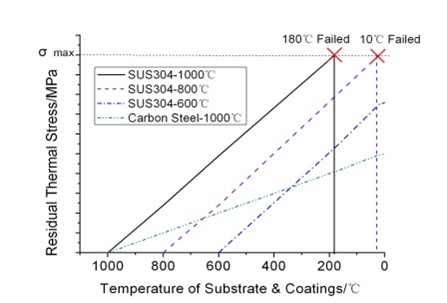
\includegraphics[
      height=0.2\textheight
      ]{subfig1.jpg}
      \subcaption{粗粉涂层}\label{fig:a}
  \end{minipage}
  \begin{minipage}{0.4\linewidth}
    \centering
    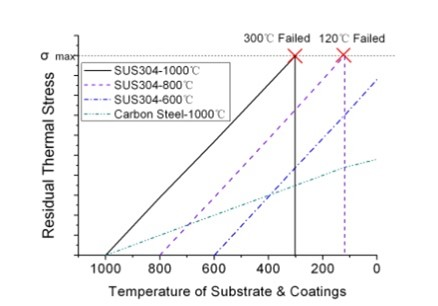
\includegraphics[
      height=0.2\textheight
      ]{subfig2.jpg}
      \subcaption{细粉涂层}\label{fig:b}
  \end{minipage}
  \caption{涂层在冷却过程中残余热应力的变化情况}
  \label{fig:figures}
\end{figure*}

\section{Pandoc Markdown结合使用}

% tex-fmt: off
本模板类的一大优势是可用极其方便地与Pandoc Markdown相结合,从而将Markdown文件方便地转化为排版好的PDF。你可以在Markdown文件开头处的YAML Header作如下指定,从而使用\texttt{uglynote}文档类,传递参数\texttt{12pt, blue}:

\begin{minted}{yaml}
documentclass: uglynote
classoptions: 12pt, blue
\end{minted}

通过\texttt{title}、\texttt{subtitle}、\texttt{author}、\texttt{date}可以设置文档的大标题、副标题、作者名字和日期。这些参数被称为Markdown文档的“元数据”。

\begin{minted}{yaml}
title: 文档标题
subtitle: 文档副标题
author: 作者的名字
date: 2025年3月11日
\end{minted}

\begin{note}
上述的这些参数在指定的时候,如果要转化为PDF via \LaTeX{} 而不转化为其他文件格式,则可以混合使用\LaTeX{}语法,例如:

\begin{minted}{yaml}
author: |
  作者的名字\thanks{
    XX研究机构,
    Email: xxx@xxxmail.com
  }
date: \zhtoday
\end{minted}
\end{note}

关于Pandoc的更多用法,另请参阅\href{https://pandoc.org/MANUAL.html}{Pandoc User's Guide}。
% tex-fmt: on

\chapter{写作示例}

\section{来自\href{https://github.com/ElegantLaTeX/}{Elegant\LaTeX}的写作示例}
我们将通过三个步骤定义可测函数的积分。首先定义非负简单函数的积分。以下设 $E$ 是 $\mathcal{R}^n$ 中的可测集。

\begin{definition}[可积性]
设 $ f(x)=\sum\limits_{i=1}^{k} a_i \chi_{A_i}(x)$ 是 $E$ 上的非负简单函数,其中 $\{A_1,A_2,\ldots$, $A_k\}$ 是 $E$ 上的一个可测分割,$a_1,a_2,\ldots,a_k$ 是非负实数。定义 $f$ 在 $E$ 上的积分为 1. 3
\begin{equation}
   \label{inter}
   \int_{E} f dx = \sum_{i=1}^k a_i m(A_i).
\end{equation}
一般情况下 $0 \leq \int_{E} f dx \leq \infty$。若 $\int_{E} f dx < \infty$,则称 $f$ 在 $E$ 上可积。
\end{definition}

一个自然的问题是,Lebesgue 积分与我们所熟悉的 Riemann 积分有什么联系和区别?之后我们将详细讨论 Riemann 积分与 Lebesgue 积分的关系。这里只看一个简单的例子。设 $D(x)$ 是区间 $[0,1]$ 上的 Dirichlet 函数。即 $D(x)=\chi_{Q_0}(x)$,其中 $Q_0$ 表示 $[0,1]$ 中的有理数的全体。根据非负简单函数积分的定义,$D(x)$ 在 $[0,1]$ 上的 Lebesgue 积分为
\begin{equation}\label{inter2}
  \int_0^1 D(x)dx = \int_0^1 \chi_{Q_0} (x) dx = m(Q_0) = 0
\end{equation}
即 $D(x)$ 在 $[0,1]$ 上是 Lebesgue 可积的并且积分值为零。但 $D(x)$ 在 $[0,1]$ 上不是 Riemann 可积的。

\begin{table}[htbp]
  \centering
  \small
  \caption{燃油效率与汽车价格}
    \begin{tabular}{lcc}
    \toprule
                  &       (1)         &        (2)      \\
    \midrule
    燃油效率      &   -238.90***      &      -49.51     \\
                  &    (53.08)        &      (86.16)    \\
    汽车重量      &                   &        1.75***  \\
                  &                   &       (0.641)   \\
    常数项        &  11253.00***      &    1946.00      \\
                  &  (1171.00)        &   (3597.00)     \\
    观测数        &     74            &      74         \\
    $R^2$         &      0.220        &       0.293     \\
    \bottomrule
    \end{tabular}%
  \label{tab:reg}%
\end{table}%

\begin{theorem}[Fubini 定理]\label{thm:fubi}
若 $f(x,y)$ 是 $\mathcal{R}^p\times\mathcal{R}^q$ 上的非负可测函数,则对几乎处处的 $x\in \mathcal{R}^p$,$f(x,y)$ 作为 $y$ 的函数是 $\mathcal{R}^q$ 上的非负可测函数,$g(x)=\int_{\mathcal{R}^q}f(x,y) dy$ 是 $\mathcal{R}^p$ 上的非负可测函数。并且
\begin{equation}\label{eq:461}
  \int_{\mathcal{R}^p\times\mathcal{R}^q} f(x,y) dxdy=\int_{\mathcal{R}^p}\left(\int_{\mathcal{R}^q}f(x,y)dy\right)dx.
\end{equation}
\end{theorem}

\begin{proof}
Let $z$ be some element of $xH \cap yH$.  Then $z = xa$ for some $a \in H$, and $z = yb$ for some $b \in H$. If $h$ is any element of $H$ then $ah \in H$ and $a^{-1}h \in H$, since $H$ is a subgroup of $G$. But $zh = x(ah)$ and $xh = z(a^{-1}h)$ for all $h \in H$. Therefore $zH \subset xH$ and $xH \subset zH$, and thus $xH = zH$.  Similarly $yH = zH$, and thus $xH = yH$, as required.
\end{proof}

回归分析 (regression analysis) 是确定两种或两种以上变量间相互依赖的定量关系的一种统计分析方法。根据定理~\ref{thm:fubi},其运用十分广泛,回归分析按照涉及的变量的多少,分为一元回归和多元回归分析;按照因变量的多少,可分为简单回归分析和多重回归分析;按照自变量和因变量之间的关系类型,可分为线性回归分析和非线性回归分析。

\begin{figure}[htbp]
  \centering
  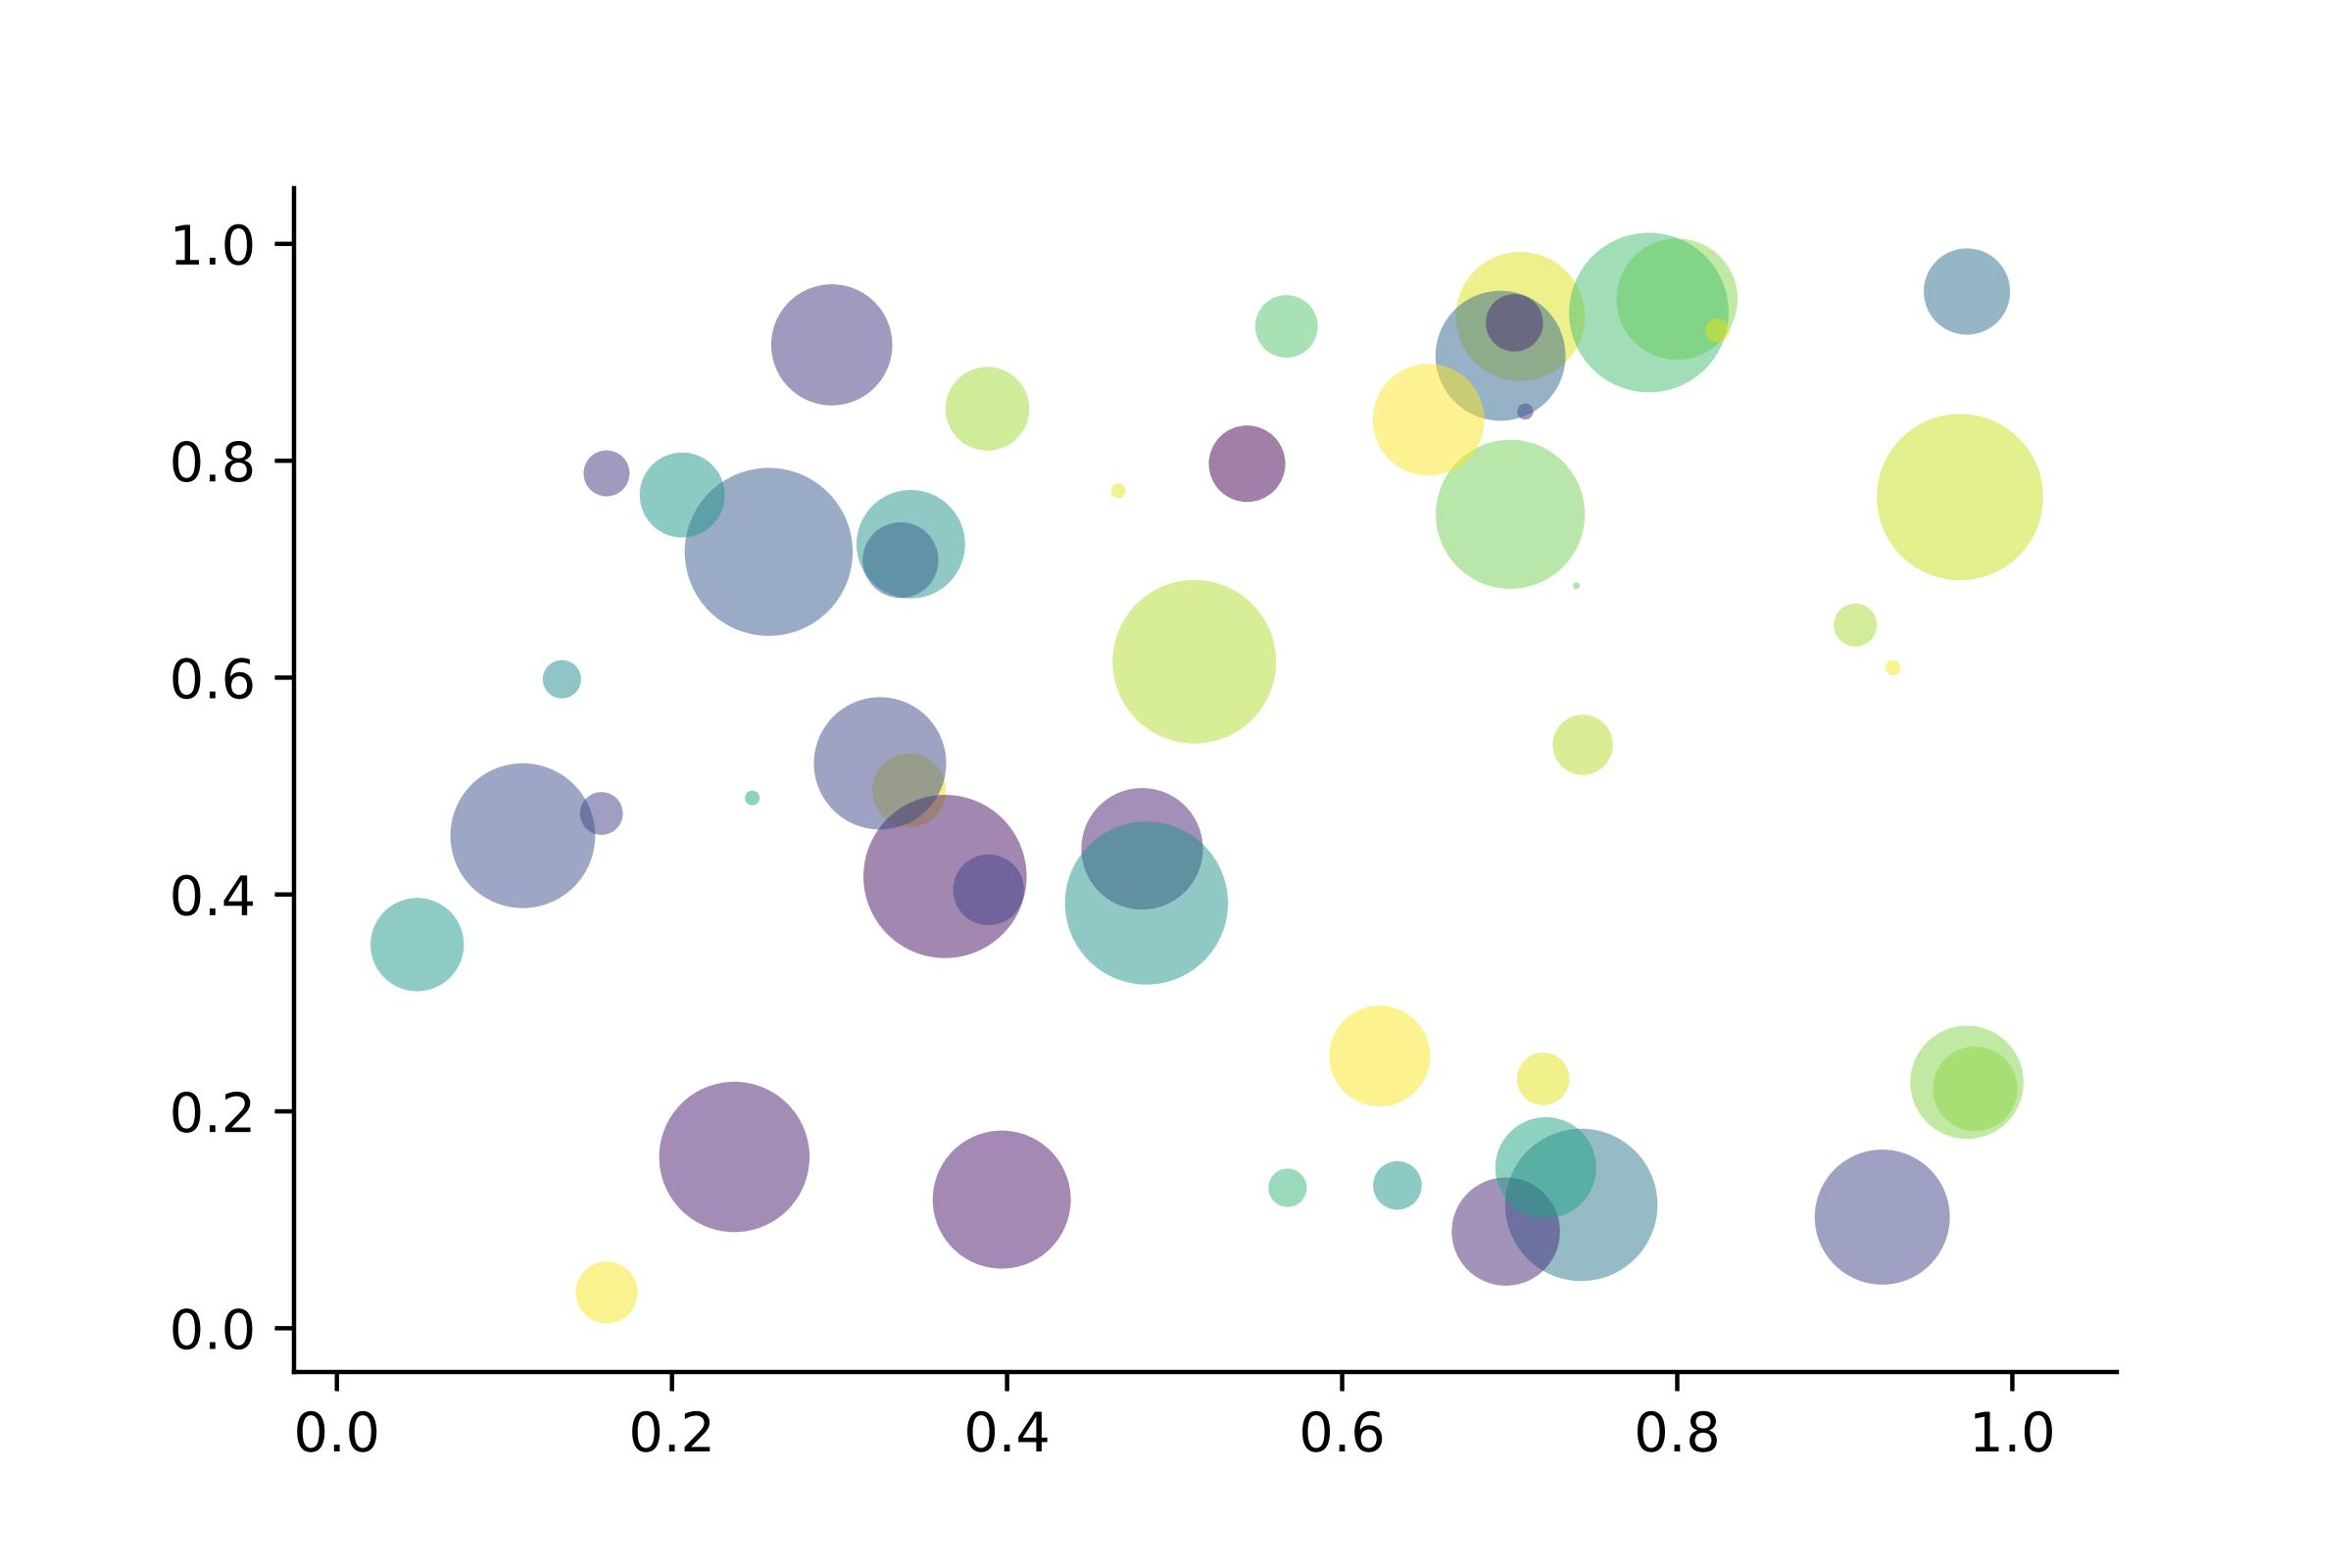
\includegraphics[width=0.75\textwidth]{scatter.jpg}
  \caption{散点图示例 $\hat{y}=a+bx$ \label{fig:scatter}}
\end{figure}

\section{更多写作示例}
\begin{example}
  在使用Miller-Tucker-Zemlin 约束作为SEC的情况下,一个典型的TSP模型的最终表述形式为:
  \begin{equation}
    \begin{array}{ll}
        \displaystyle \min f = \sum_{i=1}^n \sum_{j=1}^n d_{i, j} \times x_{i, j}, &\quad \forall (i, j) \in E, i \ne j \\
        \displaystyle \sum_{i = 1}^n x_{ij} = 1, &\quad \forall i \in V \\
        \displaystyle \sum_{j = 1}^n x_{ji} = 1, &\quad \forall j \in V \\
        \displaystyle u_i - u_j + n \cdot x_{ij} \leq n - 1, &\quad \forall (i, j) \in E, i \ne j \ne 1
        \end{array}
  \end{equation}
\end{example}

% \nocite{*}
\printbibliography[
  % heading=bibintoc, 
  title=\ebibname
]

\clearpage
\appendix
\appendixpage
\addappheadtotoc

\chapter{项目使用的宏包}
本文档类用到的所有宏包如下表\ref{tab:dependencies}所示。在使用本文档类之前,请您先确保这些宏包已经被正确配置。

\begin{table}[H]
  \centering
  \caption{本文档类所使用到的宏包}\label{tab:dependencies}
  \begin{tabular}{cccc}
    \toprule
    1 & 2 & 3 & 4 \\
    \midrule
    ifxetex & kvoptions & etoolbox & calc \\
    ctex & titling & titlesec & array \\
    hologo & geometry & fontsprc & float \\
    authblk & amsmath & amssymb & amsthm \\
    mathtools & mathrsfs & cancel & tocloft \\
    titletoc & hyperref & fancyhdr & enumerate \\
    enumitem & metalogo & setspace & caption \\
    subcaption & appendix & graphicx & booktabs \\
    multirow & longtable & pdfpages & braket \\
    qcircuit & mhchem & chemfig & tikz \\
    tikz-network & circuitikz & pdfpages & braket \\
    multirow & longtable & pgfplots & color \\
    xcolor & colortbl & xpatch & verbatim \\
    matlab-prettifier & bookmark &   &   \\
    \bottomrule
  \end{tabular}
\end{table}

\chapter{插入代码块效果示例}

\lstinputlisting[
  numbers=left, 
  language=Python, 
  caption={系统聚类方法的实现(Python):\label{lst:demo}} 
]{codes/demo.py} % Python

\end{document}